\documentclass[sigplan,10pt]{acmart}\settopmatter{printfolios=true,printccs=false,printacmref=false}

\usepackage{lineno,hyperref,xcolor}
\usepackage{flushend}
\usepackage{stmaryrd}
\usepackage{amssymb}
\usepackage{xypic}
\usepackage{semantic}
\usepackage{booktabs} 
\usepackage{subcaption}
\usepackage{enumitem}
\usepackage[shortlabels]{enumerate}
\setlist{leftmargin=6mm}

\newcounter{thc}
\newcounter{dfc}

\theoremstyle{plain}
\newtheorem{lem}[thc]{Lemma}
\newtheorem{theorem}[thc]{Theorem}

\theoremstyle{definition}
\newtheorem{definition}[dfc]{Definition}

\acmConference[PL'17]{ACM SIGPLAN Conference on Programming Languages}{January 01--03, 2017}{New York, NY, USA}
\acmYear{2017}
\acmISBN{} % \acmISBN{978-x-xxxx-xxxx-x/YY/MM}
\acmDOI{} % \acmDOI{10.1145/nnnnnnn.nnnnnnn}
\startPage{1}
\setcopyright{none}
\bibliographystyle{ACM-Reference-Format}

\title{Design and implementation of a live coding environment for data science}

\author{Tomas Petricek}
%\affiliation{
%  \institution{The Alan Turing Institute}
%  \country{London, United Kingdom}
%}
%\email{tomas@tomasp.net}


\definecolor{cmtclr}{rgb}{0.0,0.6,0.0}
\definecolor{kvdclr}{rgb}{0.0,0.0,0.6}
\definecolor{numclr}{rgb}{0.0,0.4,0.0}
\definecolor{strclr}{rgb}{0.4,0.4,0.0}
\definecolor{rstrclr}{rgb}{0.5,0.1,0.0}
\definecolor{prepclr}{rgb}{0.6,0.0,0.2}
\newcommand{\vect}[1]{\langl #1 \rangl}
\newcommand{\langl}{\begin{picture}(4.5,7)
\put(1.1,2.5){\rotatebox{60}{\line(1,0){5.5}}}
\put(1.1,2.5){\rotatebox{300}{\line(1,0){5.5}}}
\end{picture}}
\newcommand{\rangl}{\begin{picture}(4.5,7)
\put(.9,2.5){\rotatebox{120}{\line(1,0){5.5}}}
\put(.9,2.5){\rotatebox{240}{\line(1,0){5.5}}}
\end{picture}}
\newcommand{\ball}[1]{\FPeval{\result}{clip(201+#1)}\textnormal{\ding{\result}}}
\newcommand{\lsep}{~\,|\,~}
\newcommand{\num}[1]{\textcolor{numclr}{#1}}
\newcommand{\str}[1]{\textnormal{\textcolor{strclr}{\sffamily "#1"}}}
\newcommand{\rstr}[1]{\textnormal{\textcolor{rstrclr}{\sffamily "#1"}}}
\newcommand{\ident}[1]{\textnormal{\sffamily #1}}
\newcommand{\qident}[1]{\textnormal{\sffamily \guillemotleft #1\guillemotright}}
\newcommand{\dom}{\ident{dom}}
\newcommand{\kvd}[1]{\textnormal{\textcolor{kvdclr}{\sffamily #1}}}

\newcommand{\bndclr}[1]{\textcolor{kvdclr}{#1}}
\newcommand{\bkndclr}[1]{\textcolor{prepclr}{#1}}
\newcommand{\blblclr}[1]{\textcolor{numclr}{#1}}
\newcommand{\bnd}[1]{\textnormal{\textcolor{kvdclr}{\sffamily #1}}}
\newcommand{\bknd}[1]{\textnormal{\textcolor{prepclr}{\sffamily #1}}}
\newcommand{\blbl}[1]{\textnormal{\textcolor{numclr}{\sffamily #1}}}


\begin{document}
\begin{abstract}
Data science can be done by directly manipulating data using spreadsheets, or by writing 
data manipulation scripts using a programming language. The former is error-prone and
does not scale, while the latter requires expert skills. Live coding has the potential to 
bridge this gap and make writing of transparent, reproducible scripts more accessible.

In this paper, we describe a live programming environment for data science that provides instant 
previews and contextual hints, while allowing the user to edit code in an unrestricted way in
a text editor. 

Supporting a text editor is challenging as any edit can significantly change the structure of code and
fully recomputing previews after every change is too expensive. We present a technique that allows the type
checker and the interpreter to run on the fly, while code is written, and reuse results of previous 
runs. This makes it possible to efficiently provide instant feedback and live previews during development.

We formalise how programs are interpreted and how previews are computed, prove correctness
of the previews and formally specify when can previews be reused. We believe this work provides
solid and easy to reuse foundations for the emerging trend of live programming environments.
\end{abstract}
\maketitle

% ==================================================================================================
% TODO: Change values from 'n' to 'o' to indicate they are objects and can have members
% ==================================================================================================

\section{Introduction}
\label{sec:intro}

One of the aspects that make spreadsheet tools such as Excel more accessible than programming 
environments is their liveness. When you change a value in a cell in Excel \cite{spreadsheet}, the  
whole spreadsheet is updated instantly and you see the new results immediately.

Increasing number of programming environments aim to provide the same live experience for more
standard programming languages, but doing this is not easy. Fully recomputing the whole program after
every single change is inefficient and calculating how a change in source code changes the result
is extremely hard when the editor allows arbitrary manipulation of program text. For example, 
consider the following simple program that gets the release years of 10 most expensive movies 
in a data set \ident{movies}:
%
\begin{equation*}
\begin{array}{l}  
\kvd{let}~\ident{top} =\ident{movies}\\
\quad .\ident{sortBy}(\lambda x \rightarrow x.\ident{getBudget}())\ident{.take}(\num{10})\\
\quad .\ident{map}(\lambda x \rightarrow x.\ident{getReleased()}.\ident{format}(\str{yyyy}))}\\
\end{array}
\end{equation*}
%
A live coding environment shows a preview of the list of dates. Next, assume that the programmer
modifies the code by making the constant $\num{10}$ a variable and changing the date format to see 
the full date:
%
\begin{equation*}
\begin{array}{l}  
\kvd{let}~\ident{count} = \num{10}\\
\kvd{let}~\ident{top} = \ident{movies}\\
\quad .\ident{sortBy}(\lambda x \rightarrow x.\ident{getBudget}())\ident{.take}(\ident{count})\\
\quad \ident{.map}(\lambda x \rightarrow x.\ident{getReleased()}.\ident{format}(\str{dd-mm-yyyy}))}\\
\end{array}
\end{equation*}
%
Ideally, the live coding environment should understand the change, reuse a cached result of the
first two transformations (sorting and taking 10 elements) and only evaluate the last \ident{map}
to differently format the release dates of already computed top 10 movies.

This is not difficult if we represent the program in a structured way \cite{structure-based,hazelnut} 
and allow the user to edit code via known operations such as ``extract variable'' (which has
no effect on the result) or ``change constant value'' (which forces recomputation of subsequent
transformations). However, many programmers prefer to edit programs as free form text.

We present the design and implementation of a live coding system that is capable
of reusing previously evaluated expressions as in the example above, yet, is integrated into an
ordinary text editor. Our main contributions are:

\begin{itemize}[itemsep=3pt]
\item We introduce The Gamma (Section~\ref{sec:live}), a simple live coding environment for
  data science. We review its design and implementation and explain how it 
  bridges the gap between programming and spreadsheets.

\item Implementing a live programming system requires different way of thinking about compilers
  and interpreters than the one presented in classic programming language literature. Our 
  formalisation (Section~\ref{sec:formal}) captures the essence of the new perspective.

\item We formalise the evaluation of previews (Section~\ref{sec:previews}) and prove that our
  evaluation and caching mechanism is produces correct previews (Section~\ref{sec:properties-correct}) 
  and can effectively reuse partial results (Section~\ref{sec:properties-reuse}).

\item We follow the same method to implement a type checker (Section~\ref{sec:types}) for our
  language that is capable of reusing previous results. This makes it possible to efficiently support
  asynchronously provided types (Section~\ref{sec:types-providers}).

\item In more speculative conclusions (Section~\ref{sec:design}), we consider alternative
  language designs that would enable further live coding experiences, which are difficult to
  build using our current system.
\end{itemize}

\noindent
We hope the architecture and its formal presentation in this paper can contribute crucial 
foundations for the growing and important trend of text-based live coding environments.

% --------------------------------------------------------------------------------------------------

\begin{figure*}
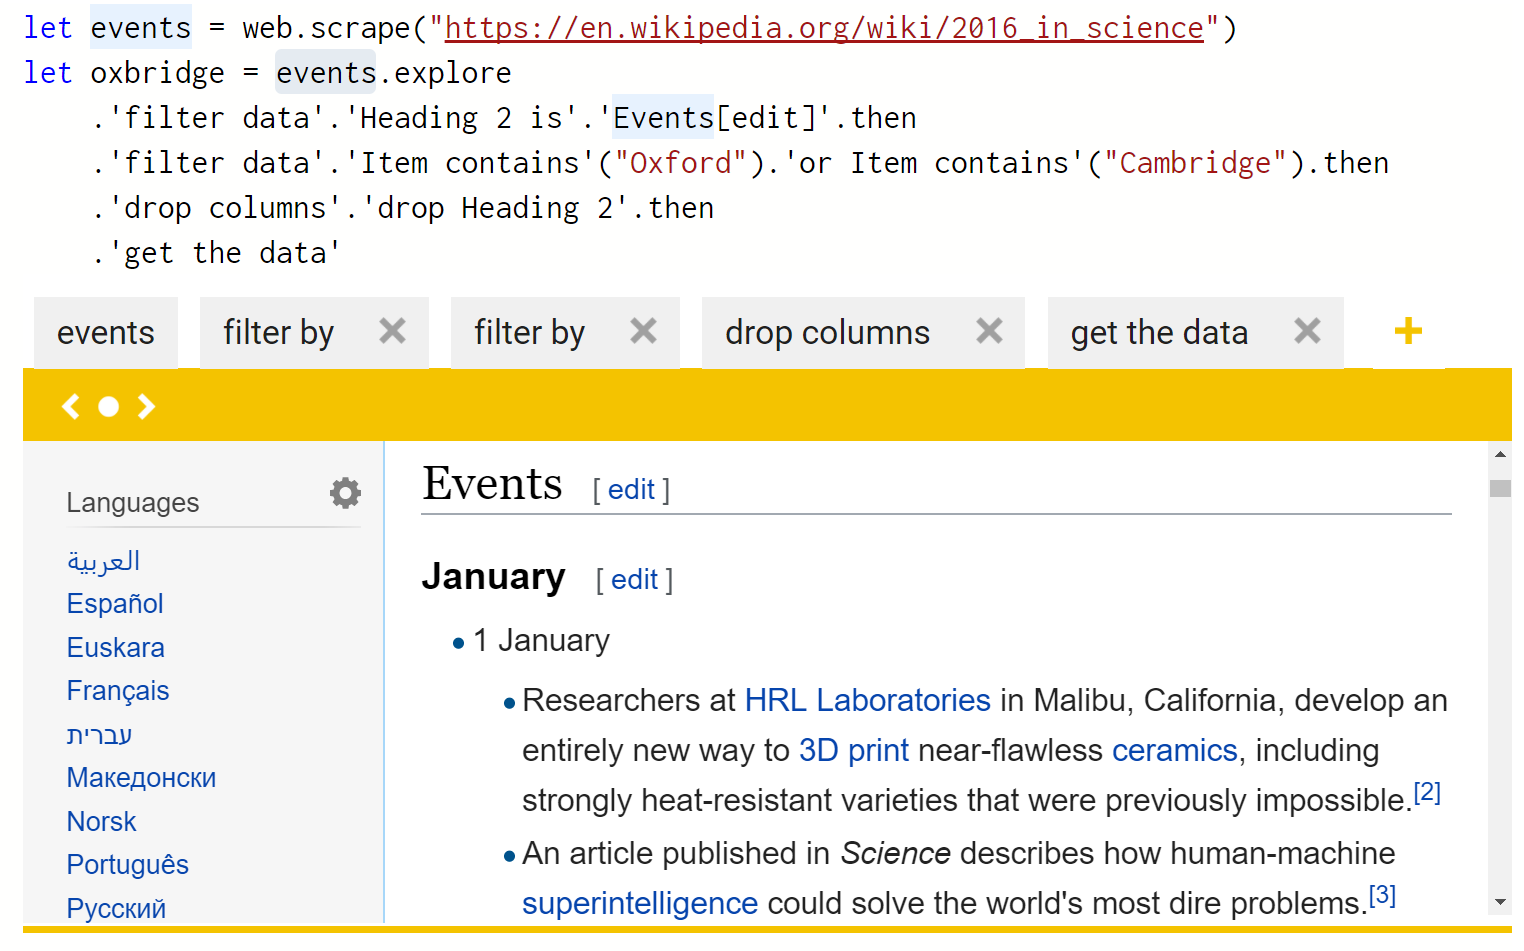
\includegraphics[scale=0.21]{wiki.png}
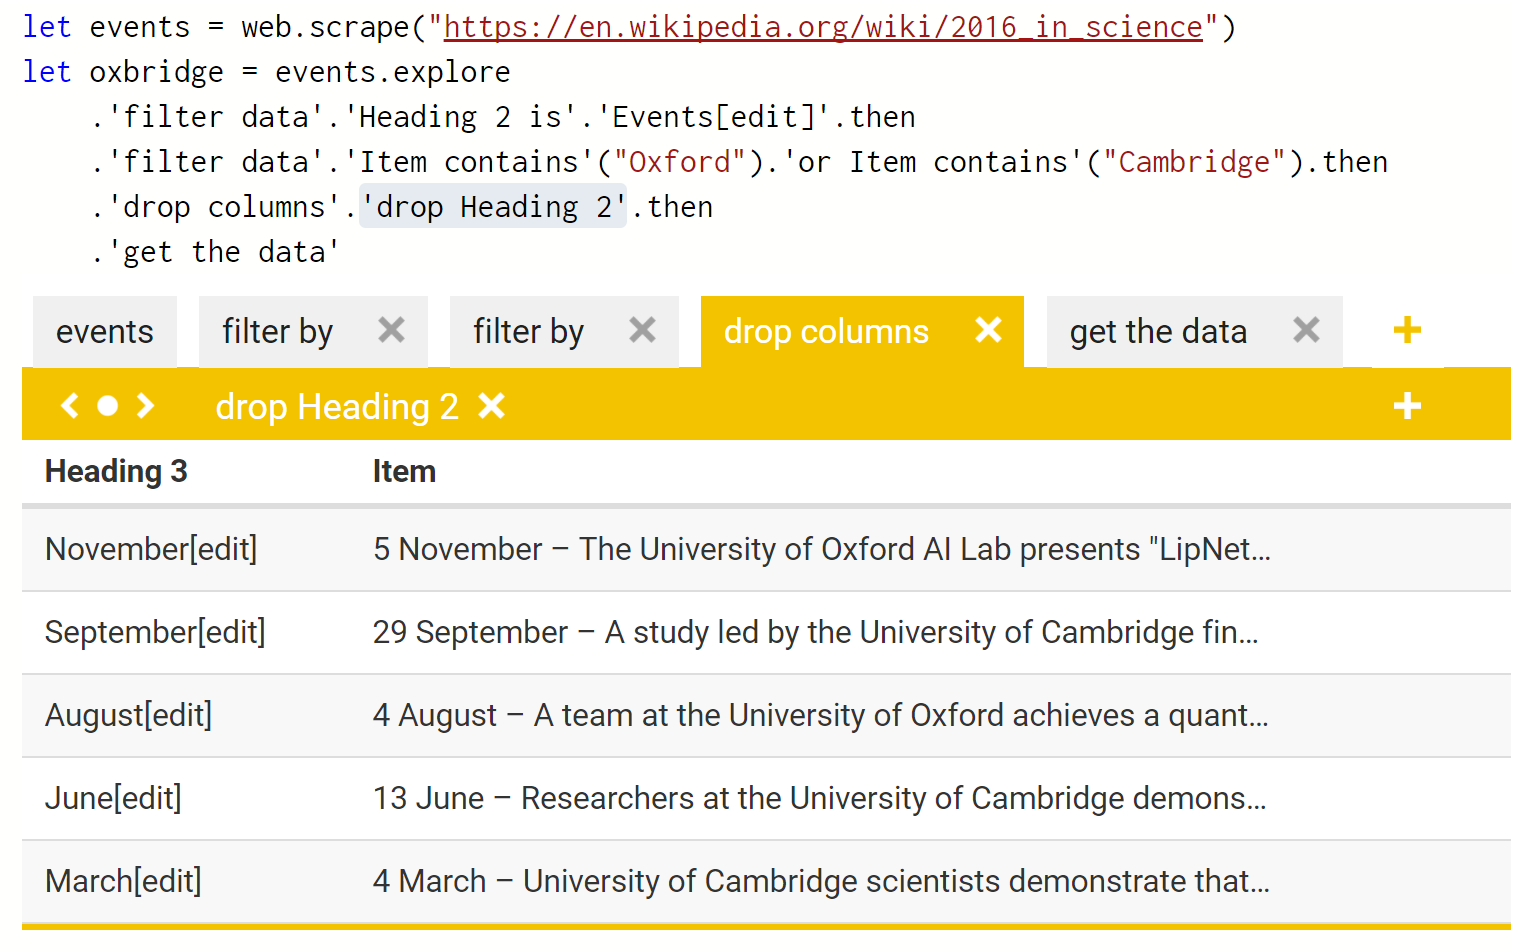
\includegraphics[scale=0.21]{drop.png}
\caption{Scraping 2016 science events. Preview of the Wikipedia source page (left) and live filtering (right).}
\label{fig:thegamma}
\end{figure*}

% ==================================================================================================

\section{Live programming for data exploration}
\label{sec:live}

The Gamma aims to make basic data exploration accessible to non-experts, such as data journalists \cite{ddj}, 
who need to use data transparently. As such, we focus on simple scripts that can be written using
tools such as Jupyter notebooks \cite{jupyter}. Those scripts follow a typical data science workflow \cite{workflow};
they acquire and reformat data, run a number of analyses using the clean data and then create 
several visualizations.

An important property of data science workflow is that we work with readily available concrete data.
Data scientists load inputs into memory and refer to it in subsequent REPL interactions. They might 
later wrap completed working code into a function (and run on multiple datasets), but 
do not start with functions. We reflect this pattern in our language. 

In this section, we provide a brief overview of The Gamma, a simple live coding environment for
data science. We discuss the language, type providers and the user interface,
before focusing on the algorithms behind live previews in Section~\ref{sec:formal}.

\subsection{The Gamma scripting language}
Figure~\ref{fig:thegamma} shows The Gamma script that scrapes items from a Wikipedia page, 
collects those marked as ``Events'' and filters them. The script illustrates two aspects of the
scripting language used by The Gamma -- its structure and its use of type providers for
dot-driven data exploration.

The scripting language is not intended to be as expressive as, say, R or Python and so it
has a very simple structure -- scripts are a sequence of let-bindings (that obtain or transform 
data) or statements (that produce visualizations). This reflects the fact that we always work
with concrete data and allows us to provide previews.

The most notable limitation of The Gamma is that the scripting language does not support top-level 
functions. This is not a problem for the simple scripts we consider, but it would be an issue for
a general-purpose language. We discuss potential design for functions that would still be based
on working with concrete data in Section~\ref{sec:design}.

\subsection{Dot-driven data exploration}

As illustrated by the second let binding in Figure~\ref{fig:thegamma}, many operations
in The Gamma can be expressed using member access via dot. The underlying mechanism is based
on type providers \cite{providers-fsharp,providers-idris}. The specific type provider used in 
the above example has been described elsewhere \cite{gamma}.

Given a data source (scraped Wikipedia page), the type provider generates type with members that allow
a range of transformations of the data such as grouping, sorting and filtering. Some of the members
are based only on the schema (e.g.~\ident{\textquotesingle Item Contains\textquotesingle} or 
\ident{\textquotesingle Drop Heading 2\textquotesingle}), but some may also be generated based
on (a sample of) the dataset (e.g.~the second member in \ident{\textquotesingle Heading 2 
is\textquotesingle.\textquotesingle Events[edit]\textquotesingle}). 

What matters for the purpose of this paper is 
the fact that most operations are expressed via member access matters. First, it means 
that we need to provide live previews for sub-expressions formed by a chain of member accesses.
Second, it means that the result of any member access expression depends on the instance and,
possibly, on the parameters provided for a method call.

\subsection{Direct manipulation and live previews}
The screenshot in Figure~\ref{fig:thegamma} show the editor as implemented in The Gamma. This
includes live previews (discussed in this paper), but also an editor that provides spreadsheet-like
interface for editing the data transformation script.

In our implementation, previews appears below the currently selected let binding.
The preview can be of several types such as web page (left) or data table (right). In this paper,
we describe how we evaluate scripts to obtain the resulting object and we ignore how such objects
are rendered.

The Figure~\ref{fig:thegamma} also shows a special handling of expressions constructed using the
pivot type provider. The editor recognises individual data transformations and provides a simple
user interface for adding and removing transformations and changing their parameters that changes
the source code accordingly. This aspect is not discussed in the present paper. 

% ==================================================================================================

\begin{figure*}
\begin{equation*}
\begin{array}{l}
\xymatrix{
& \bnd{val}(\num{10}) &\qquad\quad& \bnd{val}(\num{15})\\
\bnd{var}(\ident{data}) & 
  \bnd{mem}(\ident{skip},s_0)\ar[l]_{\blbl{arg}(0)} \ar[u]^{\blbl{arg}(1)} && 
  \bnd{mem}(\ident{take},s_1)\ar[ll]_{\blbl{arg}(0)} \ar[u]_{\blbl{arg}(1)}
}\\[5em]
\xymatrix{
&& \bnd{val}(\num{10})\\
\bnd{var}(\ident{data}) & 
  \bnd{mem}(\ident{skip}, s_0)\ar[l]_{\blbl{arg}(0)} \ar@/^/[ru]^{\blbl{arg}(1)} && 
  \bnd{mem}(\ident{take}, s_2)\ar[ll]_{\blbl{arg}(0)} \ar@/_/[lu]_{\blbl{arg}(1)}
}
\end{array}\qquad
\begin{array}{l}
\textnormal{a.) The first graph is constructed from}\\
\textnormal{the following initial expression:}\\[0.5em]
\quad\kvd{let}~x = \num{15}~\kvd{in}\\
\quad\ident{data.skip}(\num{10}).\ident{take}(x)\\
\\
\textnormal{b.) The second diagram shows the updated graph}\\
\textnormal{after the programmer changes $x$ to $10$:}\\[0.5em]
\quad\kvd{let}~x = \num{10}~\kvd{in}\\
\quad\ident{data.skip}(\num{10}).\ident{take}(x)
\end{array}
\end{equation*}
\caption{Dependency graphs formed by two steps of the live programming process. }
\label{fig:dep-graph}
\end{figure*}

% --------------------------------------------------------------------------------------------------

\newpage


\section{Formalising live coding infrastructure}
\label{sec:formal}

In this section, we present a formalisation of a live coding infrastructure for a small,
expression-based programming language that supports \kvd{let} binding, member invocations
and $\lambda$ abstractions. This is the necessary minimum for data exploration as described
in the previous section.  

It excludes constructs such as a mechanism for defining new objects as we assume that those
are imported from the context through a mechanism such as type providers.
%
\begin{equation*}
\begin{array}{lcl}
e &=& \kvd{let}~x = e~\kvd{in}~e ~|~ \lambda x\rightarrow e ~|~ e.m(e, \ldots, e) ~|~ x ~|~ n
\end{array}
\end{equation*}
%
Here, $m$ ranges over member names, $x$ over variables and $n$ over primitive values such as 
numbers. Function values can be passed as arguments to methods (provided by a type provider), but 
for the purpose of this paper, we do not need to be able to invoke them directly.

\paragraph{The problem with functions.}
In the context of live programming, \kvd{let} binding and member access are unproblematic.
We can evaluate them and provide live preview for both of them, including all their sub-expressions.
Function values are more problematic, because their sub-expressions cannot be evaluated. For example:
%
\begin{equation*}
\begin{array}{l}
\kvd{let}~\ident{page} = \lambda x \rightarrow \ident{movies}.\ident{skip}(x*\num{10}).\ident{take}(\num{10})
\end{array}
\end{equation*}
%
We can provide live preview for the \ident{movies} sub-expression, but not for 
$\ident{movies}.\ident{skip}(x*\num{10})$ because we cannot obtain the value of $x$ without
running the rest of the program and analysing how the function is called later.

The method described in this paper obtains delayed previews for sub-expressions that contain
free variables (which could be fully evaluated if values for free variables were provided), but
we describe a more speculative design of live coding friendly functions in Section~\ref{sec:design}.

% --------------------------------------------------------------------------------------------------

\subsection{Maintaining dependency graph}
\label{sec:formal-deps}

The key idea behind our implementation is to maintain a dependency graph \cite{dependencies} with 
nodes representing individual operations of the computation that can be partially evaluated
to obtain a preview. Each time the program text is modified, we parse it afresh (using an
error-recovering parser) and bind the abstract syntax tree to the dependency graph.

We remember the previously created nodes of the graph. When binding a new expression to
the graph, we reuse previously created nodes that have the same dependencies. For
expressions that have a new structure, we create new nodes (using a fresh symbol to 
identify them). 

The nodes of the graph serve as unique keys into a lookup table with previously
evaluated operations of the computation. When a preview is requested, we use the node
bound to the expression to find a preview, or evaluate it by first forcing the evaluation 
of all parents in the dependency graph.


% --------------------------------------------------------------------------------------------------

\begin{figure*}[t]
\begin{equation*}
\begin{array}{ll}
\ident{bind}_{\Gamma, \Delta}(e_0.m(e_1, \ldots, e_n)) = &(1)~~\\ 
\qquad \bndclr{v}, (\{\bndclr{v}\} \cup V_0 \cup \ldots \cup V_n, E \cup E_0 \cup \ldots \cup E_n)\\
\quad \textnormal{when}~\bndclr{v_i}, (V_i, E_i) = \ident{bind}_{\Gamma, \Delta}(e_i)\\
\quad \textnormal{and}~\bndclr{v} = \Delta(\bknd{mem}(m),[(\bndclr{v_0}, \blbl{arg}(0)), \ldots, (\bndclr{v_n}, \blbl{arg}(n))])\\
\quad \textnormal{let}~E = \{ (\bndclr{v}, \bndclr{v_0}, \blbl{arg}(0)), \ldots, (\bndclr{v}, \bndclr{v_n}, \blbl{arg}(n))\}
\\[1em]
\ident{bind}_{\Gamma, \Delta}(e_0.m(e_1, \ldots, e_n)) = &(2)\\ 
\qquad \bndclr{v}, (\{\bndclr{v}\} \cup V_0 \cup \ldots \cup V_n, E \cup E_0 \cup \ldots \cup E_n)\\
\quad \textnormal{when}~\bndclr{v_i}, (V_i, E_i) = \ident{bind}_{\Gamma, \Delta}(e_i)\\
\quad \textnormal{and}~(\bknd{mem}(m),[(\bndclr{v_0}, \blbl{arg}(0)), \ldots, (\bndclr{v_n}, \blbl{arg}(n))]) \notin \ident{dom}(\Delta)\hspace{-200em}.\\
\quad \textnormal{let}~\bndclr{v} = \bnd{mem}(m, s), s~\textnormal{fresh}\\
\quad \textnormal{let}~E = \{ (\bndclr{v}, \bndclr{v_0}, \blbl{arg}(0)), \ldots, (\bndclr{v},\bndclr{v_n}, \blbl{arg}(n)) \}
\\[1em]
\ident{bind}_{\Gamma, \Delta}(\kvd{let}~x=e_1~\kvd{in}~e_2) = \bndclr{v}, (\{\bndclr{v}\} \cup V \cup V_1, E \cup E_1)&(3)\\
\quad \textnormal{let}~\bndclr{v_1}, (V_1,E_1) = \ident{bind}_{\Gamma,\Delta}(e_1)\\
\quad \textnormal{let}~\Gamma_1 = \Gamma \cup \{(x,\bndclr{v_1})\} \\
\quad \textnormal{let}~\bndclr{v}, (V, E) = \ident{bind}_{\Gamma_1, \Delta}(e_2)
\end{array}
\begin{array}{ll}
\ident{bind}_{\Gamma, \Delta}(n) = \bnd{val}(n), (\{ \bnd{val}(n) \}, \emptyset) }&(4)
\\[1em]
\ident{bind}_{\Gamma, \Delta}(x) = \bndclr{v}, (\{ \bndclr{v} \}, \emptyset)\quad \textnormal{when}~\bndclr{v} = \Gamma(x)&(5)
\\[1.25em]
\ident{bind}_{\Gamma, \Delta}(\lambda x \rightarrow e) = \bndclr{v}, (\{\bndclr{v}\} \cup V, \{e\} \cup E)&(6)\\
\quad \textnormal{when}~\Gamma_1 = \Gamma \cup \{ x, \bnd{var}(x) \}\\
\quad \textnormal{and}~\bndclr{v_0}, (V, E) = \ident{bind}_{\Gamma_1, \Delta}(e)\\
\quad \textnormal{and}~\bndclr{v} = \Delta(\bknd{fun}(x),[(\bndclr{v_0}, \blbl{body})])\\
\quad \textnormal{let}~e = (\bndclr{v}, \bndclr{v_0}, \blbl{body}) 
\\[1.25em]
\ident{bind}_{\Gamma, \Delta}(\lambda x \rightarrow e) = \bndclr{v}, (\{\bndclr{v}\} \cup V, \{e\} \cup E)&(7)\\
\quad \textnormal{when}~\Gamma_1 = \Gamma \cup \{ x, \bnd{var}(x) \}\\
\quad \textnormal{and}~\bndclr{v_0}, (V, E) = \ident{bind}_{\Gamma_1, \Delta}(e)\\
\quad \textnormal{and}~(\bknd{fun}(x),[(\bndclr{v_0}, \blbl{body})])\notin \ident{dom}(\Delta)\\
\quad \textnormal{let}~\bndclr{v} = \bnd{fun}(x, s), s~\textnormal{fresh}\\
\quad \textnormal{let}~e = (\bndclr{v},\bndclr{v_0},\blbl{body}) 
\\[0.75em]
\end{array}
\end{equation*}
\caption{Rules of the binding process, which constructs a dependency graph for an expression.}
\label{fig:binding-rules}
\end{figure*}

% --------------------------------------------------------------------------------------------------
\paragraph{Elements of the graph.} The nodes of the graph represent individual operations
to be computed. In our design, the nodes themselves are used as keys, so we attach a unique 
\emph{symbol} to some of the nodes. That way, we can create two unique nodes representing, 
for example, access to a member named \ident{take} which differ in their dependencies.

Furthermore, the graph edges are labeled with labels indicating the kind of dependency. For
a method call, the labels are ``first argument'', ``second argument'' and so on. Formally:
%
\begin{equation*}
\begin{array}{rcll}
s&\hspace{-0.25em}\in\hspace{-0.25em}& \textit{Symbol}\\
i&\hspace{-0.25em}\in\hspace{-0.25em}& \textit{Integer}\\
n&\hspace{-0.25em}\in\hspace{-0.25em}& \textit{Primitive values}\\
x&\hspace{-0.25em}\in\hspace{-0.25em}& \textit{Variable names}\\
m&\hspace{-0.25em}\in\hspace{-0.25em}& \textit{Member names}\\[0.5em]
\bndclr{v}&\hspace{-0.25em}\in\hspace{-0.25em}&\bnd{val}(n)~|~\bnd{var}(x)~|~\bnd{mem}(m, s)~|~\bnd{fun}(x, s)&(\textit{Vertices})\\
\blblclr{l}&\hspace{-0.25em}\in\hspace{-0.25em}&\blbl{body}~|~\blbl{arg}(i)&(\textit{Edge labels})\\
\end{array}
\end{equation*}
%
The \bnd{val} node represents a primitive value and contains the value itself. Two occurrences
of $\num{10}$ in the source code will be represented by the same node. Member access \bnd{mem}
contains the member name, together with a unique symbol -- two member access nodes with different 
dependencies will contain a different symbol. Dependencies of member access are labeled with 
\blbl{arg} indicating the index of the argument (the instance has index $0$ and arguments 
start with $1$).

Finally, nodes \bnd{fun} and \bnd{var} represent function values and variables bound by $\lambda$ 
abstraction. For simplicity, we use variable names rather than de Bruijn indices and so 
renaming a bound variable forces recomputation.

\paragraph{Example graph.} Figure~\ref{fig:dep-graph} illustrates how we construct and update the 
dependency graph. Node representing $\ident{take}(x)$ depends on the argument -- the
number $\num{15}$ -- and the instance, which is a node representing $\ident{skip}(\num{10})$.
This, in turn, depends on the instance \ident{data} and the number $\num{10}$. Note that variables
bound via \kvd{let} binding such as $x$ do not appear as $\bnd{var}$ nodes. The node using it
depends directly on the node representing the result of the expression that is assigned to $x$.

After changing the value of $x$, we create a new graph. The dependencies of the node 
$\bnd{mem}(\ident{skip}, s_0)$ are unchanged and so the node is reused. This means that this
part of the program is not recomputed. The $\blbl{arg}(1)$ dependency of the \ident{take} call 
changed and so we create a node $\bnd{mem}(\ident{skip}, s_2)$ with a new fresh symbol $s_2$.
The preview for this node is then recomputed as needed using the already known values of its
dependencies.

% --------------------------------------------------------------------------------------------------

\paragraph{Reusing graph nodes.} The binding process takes an expression and constructs a 
dependency graph, reusing existing nodes when possible. For this, we keep a lookup table 
of member access and function value nodes. The key is formed by a node kind (for 
disambiguation) together with a list of dependencies. A node kind is a member access or a function:
%
\begin{equation*}
\begin{array}{lcll}
\bkndclr{k}&\in&\bknd{fun}(x)~|~\bknd{mem}(m)&\qquad(\textit{Node  kinds})
\end{array}
\end{equation*}
%
Given a lookup table $\Delta$, we write $\Delta(\bkndclr{k}, [(\bndclr{n_1},\blblclr{l_1}), \ldots,
(\bndclr{v_n},\blblclr{l_n})])$ to perform a lookup for a node of a kind $\bkndclr{k}$ that has dependencies
$\bndclr{v_1}, \ldots, \bndclr{v_n}$ labeled with labels $\blblclr{l_1}, \ldots, \blblclr{l_n}$.

For example, when creating the graph in Figure~\ref{fig:dep-graph} (b), we perform the following
lookup for the \ident{skip} member access:
%
\[ \Delta(\bknd{mem}(\ident{skip}), [(\bnd{var}(\ident{data}),\blbl{arg}(0)), (\bnd{val}(\num{10}), \blbl{arg}(1))]) \]
%
The lookup returns the node $\bnd{mem}(\ident{skip}, s_0)$ known from the previous step. We then perform
the following lookup for the \ident{take} member access:
%
\[ \Delta(\bknd{mem}(\ident{take}), [(\bnd{mem}(\ident{skip}, s_0),\blbl{arg}(0)), (\bnd{val}(\num{10}), \blbl{arg}(1))]) \]
%
In the previous graph, the argument of \ident{take} was $\num{15}$ rather than $\num{10}$ and so
this lookup fails. We then construct a new node $\bnd{mem}(\ident{take}, s_2)$ using a fresh
symbol $s_2$.

% --------------------------------------------------------------------------------------------------

\subsection{Binding an expressions to a graph}
\label{sec:formal-bind}

When constructing the dependency graph, our implementation annotates the nodes of the 
abstract syntax tree with the nodes of the dependency graph, forming a mapping
$e \rightarrow \bndclr{v}$. For this reason, we call the process \emph{binding}.

The process of binding is defined by the rules in Figure~\ref{fig:binding-rules}.
The \ident{bind} function is annotated with a lookup table $\Delta$ discussed in 
Section~\ref{sec:formal-deps} and a variable context $\Gamma$. The variable context 
is a map from variable names to dependency graph nodes and is used for variables bound
using \kvd{let} binding.

When applied on an expression $e$, binding $\ident{bind}_{\Gamma,\Delta}(e)$ returns a
dependency graph $(V, E)$ paired with a node $\bndclr{v}$ corresponding to the expression $e$.
In the graph, $V$ is a set of nodes $\bndclr{v}$ and $E$ is a set of labeled edges
$(\bndclr{v_1}, \bndclr{v_2}, \blblclr{l})$. We attach the label directly to the edge rather than
keeping a separate colouring function as this makes the formalisation simpler.

\paragraph{Binding member access.} In all rules, we recursively bind sub-expressions to get
a dependency graph for each sub-expression and a graph node that represents it. The nodes 
representing sub-expressions are then used as dependencies for lookup into $\Delta$, together
with their labels. When binding a member access, we reuse an existing node if it is defined by 
$\Delta$ (1) or we create a new node containing a fresh symbol when the domain of $\Delta$ does 
not contain a key describing the current member access~(2). 

\paragraph{Binding let binding.} For \kvd{let} binding (3), we first bind the expression $e_1$ assigned
to the variable to obtain a graph node $\bndclr{v_1}$. We then bind the body expression $e_2$,
but using a variable context $\Gamma_1$ that maps the value of the variable to the graph node
$\bndclr{v_1}$. The variable context is used when binding a variable (6) and so all variables 
declared using \kvd{let} binding will be bound to a graph node representing the value assigned 
to the variable. The node bound to the overall \kvd{let} expression is then the graph node bound
to the body expression.

\paragraph{Binding function values.} If a function value uses its argument, we will not be able
to evaluate its body. In this case, the graph node bound to a function will depend on a synthetic
node $\bnd{var}(x)$ that represents the variable with no value. When binding a function, we 
create the synthetic variable and add it to the variable context $\Gamma_1$ before binding the
body. As with member access, the node representing a function may (7) or may not (8) be already 
present in the lookup table.

% --------------------------------------------------------------------------------------------------

\begin{figure}[!b]  
\begin{equation*}
\begin{array}{l}
\ident{update}_{V,E}(\Delta_{i-1}) = \Delta_i~\textnormal{such that:}
\\[0.75em]
\quad\Delta_{i}(\bknd{mem}(m), [(\bndclr{v_0},\blbl{arg}(0)),\ldots, (\bndclr{v_n},\blbl{arg}(n))]) = \bnd{mem}(m, s)\\
\quad\quad \textnormal{for all}~\bnd{mem}(m, s) \in V\\
\quad\quad \textnormal{such that}~(\bnd{mem}(m, s), \bndclr{v_i}, \blbl{arg}(i)) \in E~\textnormal{for}~i\in 0,..,n
\\[0.75em]
\quad\Delta_{i}(\bknd{fun}(x), [(\bndclr{v_1},\blbl{body})]) = \bnd{fun}(x, s)\\
\quad\quad \textnormal{for all}~\bnd{fun}(x, s) \in V\\
\quad\quad \textnormal{such that}~(\bnd{fun}(x, s), \bndclr{v_1}, \blbl{body}) \in E
\\[0.75em]
\quad\Delta_{i}(\bkndclr{v}) = \Delta_{i-1}(\bkndclr{v})\quad \textnormal{(otherwise)}
\end{array}
\end{equation*}
\caption{Updating the node cache after binding a new graph}
\label{fig:loop}
\vspace{0.5em}
\end{figure}

% --------------------------------------------------------------------------------------------------

\begin{figure*}
\begin{equation*}
\qquad\qquad\quad\begin{array}{l}
\inference[(lift-expr)~]
  {\bndclr{v} \Downarrow \llbracket e \rrbracket_\Gamma}
  {\bndclr{v} \Downarrow_{\ident{lift}} \llbracket e \rrbracket_\Gamma}
\\
\\
\inference[(lift-prev)~]
  {\bndclr{v} \Downarrow p}
  {\bndclr{v} \Downarrow_{\ident{lift}} \llbracket p \rrbracket_\emptyset}
\\
\\
\inference[(val)~]
  {~}
  {\bnd{val}(n) \Downarrow n }
\\
\\
\inference[(var)~]
  {~}
  {\bnd{var}(x) \Downarrow \llbracket x \rrbracket_x}
  \\[0.5em]~
\end{array}
\qquad
\begin{array}{l}
\inference[(fun-val)~]
  { (\bnd{fun}(x, s), \bndclr{v}, \blbl{body}) \in E & \bndclr{v} \Downarrow p }
  { \bnd{fun}(x, s) \Downarrow \lambda x\rightarrow p }
\\
\\
\inference[(fun-bind)~]
  { (\bnd{fun}(x, s), \bndclr{v}, \blbl{body}) \in E & \bndclr{v} \Downarrow \llbracket e \rrbracket_{x} }
  { \bnd{fun}(x, s) \Downarrow \lambda x\rightarrow e }
\\
\\
\inference[(fun-expr)~]
  { (\bnd{fun}(x, s), \bndclr{v}, \blbl{body}) \in E & \bndclr{v} \Downarrow \llbracket e \rrbracket_{x,\Gamma} }
  { \bnd{fun}(x, s) \Downarrow \llbracket \lambda x\rightarrow e \rrbracket_\Gamma }
\\[0.5em]~
\end{array}
\end{equation*}
\begin{equation*}  
\qquad\qquad\begin{array}{l}
\inference[(mem-val)~]
  { \forall i\in\{0\ldots k\}.(\bnd{mem}(m, s), \bndclr{v_i}, \blbl{arg}(i)) \in E & \bndclr{v_i} \Downarrow p_i 
    & p_0.m(p_1, \ldots, p_k) \rightsquigarrow p }
  { \bnd{mem}(m, s) \Downarrow p }
\\  
\\
\inference[(mem-expr)~]
  { \forall i\in\{0\ldots k\}.(\bnd{mem}(m, s), \bndclr{v_i}, \blbl{arg}(i)) \in E & \exists j\in\{0\ldots k\}.\bndclr{v_j}\diagup\hspace{-1em}\Downarrow p_j
   & \bndclr{v_i} \Downarrow_{\ident{lift}} \llbracket e_i \rrbracket_{\Gamma_i}  }
  { \bnd{mem}(m, s) \Downarrow \llbracket e_0.m(e_1, \ldots, e_k) \rrbracket_{\Gamma_0,\ldots,\Gamma k} }
\\
\end{array}
\end{equation*}

\caption{Rules that define evaluation of previews over a dependency graph for an expression}  
\label{fig:eval}
\end{figure*}

% --------------------------------------------------------------------------------------------------


\subsection{Edit and rebind loop}

The binding process formalised in Section~\ref{sec:formal-bind} specifies how to update the 
dependency graph after updated program text is parsed. During live coding, this is done 
repeatedly as the programmer edits code. Throughout the process, we maintain a series of 
lookup table states $\Delta_0, \Delta_1, \Delta_2, \ldots$. Initially, the lookup table is 
empty, i.e.~$\Delta_0 = \emptyset$.

At a step $i$, we parse an expression $e_i$ and calculate the new dependency graph and a node
bound to the top-level expression using the previous $\Delta$:
%
\begin{equation*}
\bndclr{v}, (V, E) = \ident{bind}_{\emptyset, \Delta_{i-1}}(e_i)
\end{equation*}
%
The new state of the node cache is then computed by adding newly created nodes from the graph
$(V, E)$ to the previous cache $\Delta_{i-1}$. This is done for function and member nodes that
contain unique symbols as defined in Figure~\ref{fig:loop}. We do not need to cache nodes
representing primitive values and variables as those do not contain symbols and will remain the
same due to the way they are constructed.

% ==================================================================================================

\section{Evaluating previews}
\label{sec:previews}

The mechanism for constructing dependency graphs defined in Section~\ref{sec:formal} makes it
possible to provide live previews when editing code without recomputing the whole program 
each time the source code changes.

The nodes in the dependency graph correspond to individual operations that will be performed
when running the program. When the dependencies of an operation do not change while editing 
code, the subsequent dependency graph will reuse a node used to represent the operation. 

Our live editor keeps a map from graph nodes to live previews, so a new preview only needs to be
computed when a new node appears in the dependency graph (and the user moves the cursor to a 
code location that corresponds to the node). This section describes how previews are evaluated.

\paragraph{Previews and delayed previews.}
As discussed in Section~\ref{sec:formal}, the body of a function cannot be easily evaluated to
a value if it uses the bound variable. We do not attempt to ``guess'' possible arguments and,
instead, provide a full preview only for sub-expressions with free variables bound by a let binding.
For a function body that uses the bound variable, we obtain a \emph{delayed preview}, which is
an expression annotated with a list of variables that need to be provided before the expression
can be evaluated. We use the following notation:
%
\begin{equation*}
\begin{array}{rcll}
p&\hspace{-0.25em}\in\hspace{-0.25em}&n~|~\lambda x\rightarrow e&\quad(\textit{Fully evaluated previews})\\
d&\hspace{-0.25em}\in\hspace{-0.25em}&p~|~\llbracket e \rrbracket_\Gamma&\quad(\textit{Evaluated and delayed previews})\\
\end{array}
\end{equation*}
%
Here, $p$ ranges over fully evaluated values. It can be either a primitive value (such as number,
string or an object) or a function value with no free variables. A possibly delayed preview $d$ 
can then be either evaluated preview $p$ or an expression $e$ that requires variables $\Gamma$.
For simplicity, we use an untyped language and so $\Gamma$ is a list of variables $x_1, \ldots, x_n$.

\paragraph{Evaluation and splicing.}
In this paper, we omit the specifics of the underlying programming language and we focus on the
live coding mechanism. However, we assume that the language is equipped with an evaluation 
reduction $e \rightsquigarrow p$ that reduces a closed expression $e$ into a value $p$.

For delayed previews, we construct a delayed expression using splicing. For example, assuming
we have a delayed previews $\llbracket e_0 \rrbracket_x$ and $\llbracket e_1 \rrbracket_y$. 
If we need to invoke a member $m$ on $e_0$ using $e_1$ as an argument, we construct a new 
delayed preview $\llbracket e_0.m(e_1) \rrbracket_{x, y}$. This operation is akin to expression
splicing from meta-programming \cite{metaml,quotations} and can be more formally captured by 
Contextual Modal Type Theory (CMTT) as outlined below.

\paragraph{Evaluation of previews.}
The evaluation of previews is defined in Figure~\ref{fig:eval}. Given a dependency graph $(V, E)$,
we define a relation $\bndclr{v}\Downarrow d$ that evaluates a sub-expression corresponding to 
the node $\bndclr{v}$ to a (possibly delayed) preview $d$. 

The auxiliary relation $\bndclr{v}\Downarrow_{\ident{lift}} d$ always evaluates
to a delayed preview. If the ordinary evaluation returns a delayed preview, so does the auxiliary
relation (\emph{lift-expr}). If the ordinary evaluation returns a value, the value is wrapped
into a delayed preview requiring no variables (\emph{lift-prev}).

Graph node representing a value is evaluated to a value (\emph{val}) and a graph node representing
an unbound variable is reduced to a delayed preview that requires the variable and returns its
value (\emph{var}).

For member access, we distinguish two cases. If all arguments evaluate to values (\emph{member-val}),
then we use the evaluation relation $\rightsquigarrow$, immediately evaluate the member access and 
produce a value. If one of the arguments is delayed (\emph{member-expr}), because the member access 
is in the body of a lambda function, then we produce a delayed member access expression that
requires the union of the variables required by the individual arguments.

The evaluation of function values is similar, but requires three cases. If the body can 
be reduced to a value with no unbound variables (\emph{fun-val}), we return a lambda function that
returns the value. If the body requires only the bound variable (\emph{fun-bind}), we return a 
lambda function with the delayed preview as the body. If the body requires further variables,
the result is a delayed preview.

\paragraph{Caching previews.}
For simplicity, the relation $\Downarrow$ in Figure~\ref{fig:eval} does not specify how previews 
are cached and linked to graph nodes. In practice, this is done by maintaining a lookup table
from graph nodes $\bdnclr{v}$ to (possibly delayed) previews $p$.
Whenever $\Downarrow$ is used to obtain a preview for a graph node, we first 
attempt to find an already evaluated preview using the lookup table. If the preview has not
been previously evaluated, we evaluate it and add it to the lookup table.

The evaluated previews can be reused in two ways. First, multiple nodes can 
depend on one sub-graph in a single dependency graph (if the same sub-expression appears
twice in the program). Second, the keys of the lookup table are graph nodes and nodes are 
reused when a new dependency graph is constructed after the user edits the source code.

\paragraph{Semantics of delayed previews.}
The focus of this paper is on the design and implementation of a live coding environment, 
but it is worth noting that the structure of delayed previews is closely linked to the work
on Contextual Modal Type Theory (CMTT) \cite{cmtt} and comonads \cite{cmtt-denotation}. 

In CMTT, $\lbrack \Psi \rbrack A$ denotes that a proposition $A$ is valid in context $\Psi$,
which is closely related to our delayed previews written as $\llbracket A \rrbracket_\Psi$.
CMTT defines rules for composing context-dependent propositions that would allow us to express
the splicing operation used in (\emph{mem-expr}). In categorical terms, the context-dependent
proposition can be modeled as an indexed comonad \cite{effectrev,graded}. The evaluation of a preview with no 
context dependencies (built implicitly into our evaluation rules) corresponds to the counit
operation of a comonad and would be explicitly written as $\llbracket A \rrbracket_\emptyset \rightarrow A$.

% ==================================================================================================

\begin{figure*}[t]
\vspace{-0.5em}
\begin{equation*}
\begin{array}{ll}
\ident{bind}_{\Gamma, \Delta, c}(e_0.m(e_1, \ldots, e_n)) = &(2b)\\ 
\qquad \bndclr{v}, (\{\bndclr{v}\} \cup V_0 \cup \ldots \cup V_n, E \cup E_0 \cup \ldots \cup E_n)\\
\quad \textnormal{when}~\bndclr{v_0}, (V_0, E_0) = \ident{bind}_{\Gamma, \Delta, \bot}(e_0)\\
\quad \textnormal{and}~c_i = (\bndclr{v_0}, \blbl{callsite}(m,i))\hspace{4.8em} (i \in 1\ldots n)\\
\quad \textnormal{and}~\bndclr{v_i}, (V_i, E_i) = \ident{bind}_{\Gamma, \Delta, c_i}(e_i)\qquad (i\in 1\ldots n)\\
\quad \textnormal{and}~(\bknd{mem}(m),[(\bndclr{v_0}, \blbl{arg}(0)), \ldots, (\bndclr{v_n}, \blbl{arg}(n))]) \notin \ident{dom}(\Delta)\hspace{-200em}.\\
\quad \textnormal{let}~\bndclr{v} = \bnd{mem}(m, s), s~\textnormal{fresh}\\
\quad \textnormal{let}~E = \{ (\bndclr{v}, \bndclr{v_0}, \blbl{arg}(0)), \ldots, (\bndclr{v},\bndclr{v_n}, \blbl{arg}(n)) \}
\end{array}
\qquad\qquad
\begin{array}{ll}
\ident{bind}_{\Gamma, \Delta, (\bndclr{v_c}, \blblclr{l_c} )}(\lambda x \rightarrow e) = \bndclr{v}, (\{\bndclr{v}\} \cup V_0, E \cup E_0)&(7b)\\
\quad \textnormal{when}~(\bknd{var}(x),[(\bndclr{v_c}, \blblclr{l_c} )])\notin \ident{dom}(\Delta)\\
\quad \textnormal{let}~\bndclr{v_x} = \bnd{var}(x, s_x), s_x~\textnormal{fresh}\\
\quad \textnormal{and}~\Gamma_1 = \Gamma \cup \{ x, \bndclr{v_x} \}\\
\quad \textnormal{and}~\bndclr{v_0}, (V_0, E_0) = \ident{bind}_{\Gamma_1, \Delta, \bot}(e)\\
\quad \textnormal{when}~(\bknd{fun}(x),[(\bndclr{v_0}, \blbl{body}), (\bndclr{v_c}, \blblclr{l_c} )])\notin \ident{dom}(\Delta)\\
\quad \textnormal{let}~\bndclr{v} = \bnd{fun}(x, s_f), s_f~\textnormal{fresh}\\
\quad \textnormal{let}~E = \{ (\bndclr{v},\bndclr{v_0},\blbl{body}), (\bndclr{v},\bndclr{v_c},\blblclr{l_c}), (\bndclr{v_x},\bndclr{v_c},\blblclr{l_c}) \}
\\[0.75em]
\end{array}
\end{equation*}
\vspace{-0.5em}
\caption{Revised binding rules, tracking call sites of function values.} 
\label{fig:binding-rules-callsite}
\vspace{-0.5em}
\end{figure*}

% ==================================================================================================

\section{Type checking}
\label{sec:types}

Evaluating live previews can be an expensive operations, so being able to cache partial previews
is a must for a live coding environment. Type checking is typically fast, so the main focus of
this paper is on live previews. However, asynchronous type providers in The Gamma (Section~\ref{sec:types-providers}) 
can make type checking time consuming, and so we use the dependency graph also for type checking
(Section~\ref{sec:types-graph}). Type checking lambda functions (Section~\ref{sec:types-funs}) 
requires a slight extension of the model discussed in Section~\ref{sec:formal}. 
   
% --------------------------------------------------------------------------------------------------

\subsection{Asynchronously provided types}
\label{sec:types-providers}

Data available in The Gamma can be defined using several kinds of type providers. The type provider
used in Figure~\ref{fig:thegamma} as asynchronous \cite{async}. It downloads the sample URL and generates 
types based on the contents of the web page. The parameter to \ident{web.scrape} is a static 
parameter and is evaluated during type-checking. We omit details in this paper, but we note this
works similarly to F\# type providers \cite{providers-fsharp}. 

Type providers can also be implemented as REST services \cite{rest} to allow anyone implement a data source
in the language of their choice. In this case, each member of a call-chain returns a type that is
generated based on the result of an HTTP request. For example, when the user types \ident{worldbank}
(to access information about countries), the type provider makes a request to   
\url{http://thegamma-services.azurewebsites.net/worldbank}, which returns two members:
%
\begin{equation*}
\begin{array}{l}
[~\{\rstr{name}\!:\str{byYear},\rstr{returns}\!:\\
~\quad \{\rstr{kind}\!:\str{nested},\rstr{endpoint}\!:\str{/pickYear}\}\}\\
\hspace{0.55em}\{\rstr{name}\!:\str{byCountry},\rstr{returns}\!:\\
~\quad \{\rstr{kind}\!:\str{nested},\rstr{endpoint}\!:\str{/pickCountry}\}\}~]
\end{array}
\end{equation*}
%
This indicates that \ident{worldbank} has members \ident{byYear} and \ident{byCountry}.
If the user types \ident{worldbank.byCountry}, a request is made to the specified URL 
\url{http://thegamma-services.azurewebsites.net/worldbank/pickCountry}:
%
\begin{equation*}
\begin{array}{l}
[~\{\rstr{name}\!:\str{Andorra},\rstr{trace}\!:[\str{"country=AR"}], \\
\quad \rstr{returns}\!:\{\rstr{kind}\!:\str{nested},\rstr{endpoint}\!:\str{/pickTopic}\}\}\\
\hspace{0.55em}\{\rstr{name}\!:\str{Afghanistan},\rstr{trace}\!:[\str{"country=AF"}],\\
\quad \rstr{returns}\!:\{\rstr{kind}\!:\str{nested},\rstr{endpoint}\!:\str{/pickTopic}\}\},\,..]
\end{array}
\end{equation*}
%
This returns a list of countries which can then be accessed as members via 
\ident{worldbank.byCountry.Andorra}, etc.

This is one reason for why type checking in The Gamma can be time consuming. Other
type providers may perform other more computationally intensive work to provide types and so
it is desirable to reuse type-checking results during live coding. The rest of this section
shows how this is done using the dependency graph discussed in Section~\ref{sec:formal}.

\begin{figure}[!b]
\vspace{-0.5em}
\begin{equation*}
\xymatrix{
&\bnd{val}(o)\\
&\bnd{mem}(m, s_0) \ar[u]_{\blbl{arg}(0)} \ar[dl]^{\blbl{arg}(1)} \\
\bnd{fun}(x, s_2) \ar@/^/[uur]^{\blbl{callsite}(m, 1)} \ar[rr]^{\blbl{body}} && \bnd{var}(x, s_1) \ar@/_/[uul]_{\blbl{callsite}(m, 1)}
}  
\end{equation*}
\caption{Dependency graph for $o.m(\lambda x\rightarrow x)$}
\label{fig:graph-func}
\end{figure}

% --------------------------------------------------------------------------------------------------

\subsection{Revised binding of functions}
\label{sec:types-funs}

The Gamma script supports lambda functions, but only in a limited way. A function can be passed
as a parameter to a method, which makes type checking of functions easier. For example, consider:
%
\begin{equation*}
\begin{array}{l}  
\ident{movies}.\ident{sortBy}(\lambda x \rightarrow x.\ident{getBudget}())
\end{array}
\end{equation*}
%
If \ident{movies} is a collection of \ident{Movie} objects, the type of the lambda function must be
$\ident{Movie}\rightarrow\ident{bool}$ and so the type of $x$ is \ident{Movie}. This is similar to
type checking of lambda functions in C\# \cite{csharp}, where type is also inferred from the context (or has
to be specified explicitly). 

We do not currently allow lambda functions as stand-alone let-bound 
values. This could be done by requiring explicit types, or introducing polymorphism, but it was not
necessary for the limited domain of non-expert data exploration.

\paragraph{Dependency graph for functions.}
In the binding process specified in Section~\ref{sec:formal}, a variable is a leaf of the dependency
graph. In the revised model, it depends on the context in which it appears. A new edge labeled
$\blbl{callsite}(m, i)$ indicates that the source node is the input variable of a function 
passed as the $i^\textnormal{th}$ argument to the $m$ member of the expression represented by the
target node. A node representing function is linked to the call site using the same edge.

Figure~\ref{fig:graph-func} shows the result of binding $o.m(\lambda x\rightarrow x)$. Both
$\bnd{fun}(x, s_2)$ and $\bnd{var}(x, s_1)$ now depend on the node representing $o$. The new 
$\blbl{callsite}$ edge makes it possible to type-check function and variable nodes just using their 
dependencies. As before, the member invocation $\bnd{mem}(m, s_0)$ 
depends on the instance using $\blbl{arg}(0)$ and on its argument using $\blbl{arg}(1)$. 

% --------------------------------------------------------------------------------------------------

\begin{figure*}
\vspace{0.5em}
\begin{equation*}
\begin{array}{l}
\qquad\inference[(val)~]
  {\Sigma(n) = \alpha}
  {\bnd{val}(n) \vdash \alpha }
\quad\qquad
\inference[(var)~]
  { (\bnd{var}(x,s), \bndclr{v}, \blbl{callsite}(m, i)) \in E &
    \bndclr{v} \vdash (.., m:(\tau_1, \ldots, \tau_k)\rightarrow \tau,..) & \tau_i=\tau'\rightarrow\tau'' }
  { \bnd{var}(x, s) \vdash \tau' }
\\[2.5em]
\inference[(fun)~]
  { \{(\bnd{fun}(x,s), \bndclr{v_b}, \blbl{body}), (\bnd{var}(x,s), \bndclr{v_c}, \blbl{callsite}(m, i))\} \subseteq E &
    \bndclr{v_c} \vdash (.., m:(\tau_1, \ldots, \tau_k)\rightarrow \tau,..) &
    \tau_i=\tau'\rightarrow\tau'' & \bndclr{v_b} \vdash \tau'' }
  { \bnd{fun}(x, s) \vdash \tau' \rightarrow \tau'' }
\\[2.5em]
\qquad\qquad\quad\inference[(mem)~]
  { \forall i\in\{0\ldots k\}.(\bnd{mem}(m, s), \bndclr{v_i}, \blbl{arg}(i)) \in E &
    \bndclr{v_0} \vdash (.., m:(\tau_1, \ldots, \tau_k) \rightarrow \tau, ..)& \bndclr{v_i} \vdash \tau_i }
  { \bnd{mem}(m, s) \vdash \tau }
\\[1em]
\end{array}
\end{equation*}
\caption{Rules that define evaluation of previews over a dependency graph for an expression}  
\vspace{0.5em}
\label{fig:tc}
\end{figure*}

% --------------------------------------------------------------------------------------------------

\paragraph{Revised binding process.}
For the revised binding process, we introduce a new edge label $\blbl{callsite}$. Variable nodes
now have dependencies and so we cache them and attach a symbol $s$ to \bnd{var}, so we also 
introduce a node kind $\bknd{var}$ as part of a lookup key for $\Delta$. 

The \ident{bind} function now has a parameter $c$, in addition to $\Gamma$ and $\Delta$, which 
represents the context in which the binding happens. This is either a member invocation (labeled 
with instance node $\bndclr{v}$ and \blbl{callsite} label $\blblclr{l}$), or not a member 
invocation written as $\bot$. The updated definitions are:
%
\begin{equation*}
\begin{array}{lcll}
\bndclr{v} &\hspace{-0.5em}\in\hspace{-0.5em}&\bnd{val}(n)~|~\bnd{var}(x, s)~|~\bnd{mem}(m, s)~|~\bnd{fun}(x, s)&(\textit{Vertices})\\
\blblclr{l}&\hspace{-0.5em}\in\hspace{-0.5em}&\blbl{body}~|~\blbl{arg}(i)~|~\blbl{callsite}(m,i)&(\textit{Edge labels})\\
\bkndclr{k}&\hspace{-0.5em}\in\hspace{-0.5em}&\bknd{fun}(x)~|~\bknd{mem}(m)~|~\bknd{var}(x)&(\textit{Node kinds})\\
          c&\hspace{-0.5em}\in\hspace{-0.5em}&\bot ~|~(\bndclr{v}, \blblclr{l})&(\textit{Call sites})\\
\end{array}
\end{equation*}
%
The key parts of the revised definition of the \ident{bind} function are shown in Figure~\ref{fig:binding-rules-callsite}.
We now write $\ident{bind}_{\Gamma,\Delta,c}$ where $c$ represents the context in which the
binding occurs. This is set to $\bot$ in all cases, except when binding arguments of a member call.
In (2b), we first recursively bind the instance node using $\bot$ as the context and then 
bind all the arguments using $(\bndclr{v_0}, \blbl{callsite}(m, i))$ as the context for $i^{\textnormal{th}}$ 
argument. The rest is as in case (2) before. The case (1) is updated similarly and is not shown 
here for brevity.

When binding a function (7b), we now also store variable nodes in $\Delta$ and so we check if a 
variable with the given call site exists. If no, we create a fresh node $\bnd{var}(x, s_x)$.
The node is added to $\Gamma$ as before. At the end, we now also include a call site edge from the 
variable node and from the function node in $E$. We omit a similar variant of the case (6).
The remaining cases (3)-(5) are the same, except that \ident{bind} has the additional $c$ parameter
and recursive calls always set it to $\bot$.

Finally, the \ident{update} function in Figure~\ref{fig:loop} also needs to be updated to store the
newly created \bnd{var} nodes. This is done by adding the following single case:

\begin{equation*}
\begin{array}{l}
\Delta_{i}(\bknd{var}(x), [(\bndclr{v},\blbl{callsite}(m,i))]) = \bnd{var}(x, s)\\
\quad\quad \textnormal{for all}~\bnd{var}(x, s) \in V\\
\quad\quad \textnormal{such that}~(\bnd{var}(x, s), \bndclr{v}, \blbl{callsite}(m,i)) \in E
\end{array}
\end{equation*}

% --------------------------------------------------------------------------------------------------

\subsection{Type checking over dependency graphs}
\label{sec:types-graph}

The type system for The Gamma supports a number of primitive types (such as integers and strings) 
written as $\alpha$. Composed types include functions and objects with members. Objects are be 
provided by type providers, but we omit the details here. Types of object members are written as
$\sigma$ and can have multiple arguments:
%
\begin{equation*}
\begin{array}{lcll}
\tau&\in&\alpha ~|~ \tau \rightarrow \tau ~|~ \{m_1\!:\!\sigma_1, \ldots, m_n\!:\!\sigma_n\} &\quad(\textit{Types})\\
\sigma &\in& (\tau_1, \ldots, \tau_n) \rightarrow \tau &\quad(\textit{Members})\\
\end{array}
\end{equation*}
%
The typing judgements are written in the form $\bnd{v}\vdash \tau$. They are parameterised by the
dependency graph $(V, E)$, but this is not modified during type checking so we keep it implicit
rather than writing e.g.~$\bnd{v}\vdash_{(V,E)} \tau$.

\paragraph{Type checking.}
The typing rules are shown in Figure~\ref{fig:tc}. Types of primitive values $n$ are obtained
using a global lookup table $\Sigma$ (\emph{val}). When type checking a member call (\emph{mem}),
we find its dependencies $\bndclr{v_i}$ and check that the first one (instance) is an object with 
the required member $m$. The types of input arguments of the member then need to match the types 
of the remaining (non-instance) nodes. 

Type checking a function (\emph{fun}) and a variable (\emph{var}) is similar. In both cases,
we follow the \blbl{callsite} edge to find the member that accepts the function as an argument.
We obtain the type of the function from the type of the $i^\textnormal{th}$ argument of the 
member. We use the input type as the type of variable (\emph{var}). For functions, we also check 
that the resulting type matches the type of the body (\emph{fun}).

\paragraph{Caching results.}
Performing type checking over the dependency graph, rather than over the abstract syntax tree,
enables us to reuse the results of previously type checked parts of a program. As when 
caching evaluated previews (Section~\ref{sec:previews}), we build a lookup table mapping graph
nodes to types. When type checking a node, we first check the cache and, only if it is new, 
follow the $\vdash$ relation to obtain the type. 

As a result, code can be type checked on-the-fly during editing, even when asynchronous type 
providers are used, and the programmer gets instant feedback without delays.

% ==================================================================================================

\section{Properties of live coding environment}
\label{sec:properties}

The dependency graph makes it possible to cache partial results when evaluating previews. 
The mechanism needs to satisfy two properties.
First, if we evaluate a preview using dependency graph with caching, it should be the same as the
value we would obtain by evaluating the expression directly. Second, the evaluation of previews 
using dependency graphs should -- in some cases -- reuse previously evaluated partial results.
In other words, we show that the mechanism is correct and implements a useful optimization. 

\subsection{Modeling expression evaluation}
In The Gamma language, computations are expressed using
member access, written as $e.m(e_1,\ldots, e_n)$. In this paper, we do not define how member
access evaluates. This has been done elsewhere \cite{gamma}, but more importantly, the evaluation of
previews does not rely on the exact specifics of the evaluation, provided that the language
satisfies certain basic conditions. The following definitions provides the necessary structure 
for discussing correctness of previews.

Partial evaluation may reduce an expression under $\lambda$-abstraction. We do not require that
the reduction of the host language does this. Instead, we define an extended reduction relation
and use that in the proofs. The host language only needs to compose well with such extended reduction
as captured by the \emph{compositionality} property below. We also require that the language allows
elimination of let bindings.

\begin{definition}[Host language]
\label{def:host}
Given a relation on expressions $e_1 \rightsquigarrow e_2$ that models small-step evaluation, we define:

\begin{itemize}
\item[--]  
 A \emph{preview evaluation context} (also referred to as \emph{context}):

\vspace{-1.25em}
\begin{equation*}
\begin{array}{lcl}
C[-] &\hspace{-1em}=\hspace{-1em}& \kvd{let}~x = -~\kvd{in}~e ~|~ \kvd{let}~x = e~\kvd{in}~- ~|~ \lambda x\rightarrow - \\
     &&  e_0.m(e_1, \ldots, e_{k-1}, -, e_{k+1}, \ldots e_n)
\end{array}
\end{equation*}

\item[--]  
An extended reduction relation $\rightsquigarrow_\beta$ such that, for any context $C$, 
$C[e_1] \rightsquigarrow_\beta C[e_2]$ whenever $e_1 \rightsquigarrow e_2$.

\item[--]  
Let elimination $\rightsquigarrow_\ident{let}$ such that, using  capture-avoiding substitution,
  $C[\kvd{let}~x=e_1~\kvd{in}~e_2] \rightsquigarrow_\ident{let} C[e_2[x\leftarrow e_1]]$
\end{itemize}

\noindent
We say that $\rightsquigarrow$ is a suitable \emph{host language reduction} if:
\begin{itemize}
\item[--] It satisfies the \emph{compositionality} property, that is if $e \rightsquigarrow e'$ and 
$C[e]\rightsquigarrow_\beta e''$ then also $C[e']\rightsquigarrow_\beta e''$.

\item[--] Let elimination does not affect the result, i.e.~if $e \rightsquigarrow_{\ident{let}} e'$ 
and $e'\rightsquigarrow_\beta e''$ then also $e\rightsquigarrow_\beta e''$ 
\end{itemize}
\end{definition}

\noindent
The host language in The Gamma is a simple call-by-value functional language without side-effects,
and so it satisfies both compositionality and allows let bindings to be eliminated, although the
latter affects the performance. The mechanism for preview evaluation presented here would also 
work for call-by-name languages, but it would suffer from the expected difficulties in the 
presence of side-effects or non-determinism.

% --------------------------------------------------------------------------------------------------

\subsection{Correctness of previews}
\label{sec:properties-correct}

To show that the evaluated previews are correct, we prove two properties. Correctness 
(Theorem~\ref{thm:correcntess}) guarantees that, no matter how a graph is constructed, when we use
it to evaluate a preview for an expression, the preview is the same as the value we would obtain
by evaluating the expression directly. Determinacy (Theorem~\ref{thm:determinacy}) guarantees that if
we cache a preview for a graph node and update the graph, the preview we would evaluate using the
updated graph would be the same as the cached preview. 

To simplify the proofs, we consider expressions without let bindings. This is possible, because
eliminating let bindings does not change the result in the host language (Definition~\ref{def:host})
and it also does not change the constructed dependency graph as shown in Lemma~\ref{thm:let-elimination}.

\begin{lem}[Let elimintion]
\label{thm:let-elimination}  
Given an expression $e_1$ such that $e_1 \rightsquigarrow_\ident{let} e_2$ and a lookup table $\Delta_0$
then if $\bndclr{v_1}, (V_1, E_1) = \ident{bind}_{\emptyset, \Delta_0}(e_1)$ and  
$\bndclr{v_2}, (V_2, E_2) = \ident{bind}_{\emptyset, \Delta_1}(e_2)$ such that $\Delta_1 = \ident{update}_{V_1, E_1}(\Delta_0)$
then it holds that $\bndclr{v_1} = \bndclr{v_2}$ and also $(V_1, E_1) = (V_2, E_2)$.
\end{lem}
\begin{proof}
Assume $e_1 = C[\kvd{let}~x=e'~\kvd{in}~e'']$ and the resulting $e_2 = C[e''[x\leftarrow e']]$. The case 
$\ident{bind}_{\Gamma,\Delta}(\kvd{let}~x=e'~\kvd{in}~e'')$ when binding $e_1$ is handled using
(3).

When binding $e_1$, the node resulting from binding $e'$ is added to the graph $V_1, E_1$ and is 
referenced each time $x$ is used. When binding $e_2$, the node representing $e'$ is a primitive value,
or already present in $\Delta_1$ (added by $\ident{update}_{V_1, E_1}$) and is reused each time 
$\ident{bind}_{\Gamma,\Delta_1}(e')$ is called.
\end{proof}

The Lemma~\ref{thm:let-elimination} provides a way of removing let bindings from an expression,
such that the resulting dependency graph remains the same. Here, we bind the original expression
first, which adds the node for $e'$ to $\Delta$. In our implementation, this is not needed
because $\Delta$ is updated while the graph is being constructed using $\ident{bind}$. 
To keep the formalisation simpler, we separate the process of building the dependency graph 
and updating $\Delta$. 

Now, we can show that, given a let-free expression, the preview obtained using a correctly
constructed dependency graph is the same as the one we would obtain by directly evaluating the
expression. This requires a simple auxiliary lemma and the full proof is shown in 
Appendix~\ref{sec:app-correctness}.

\begin{lem}
\label{thm:lemma-lookup}[Lookup inversion]
Given $\Delta$ obtained using \ident{update} as defined in Figure~\ref{fig:loop} then: 
\begin{itemize}
\raggedright
\item[--] If $\bndclr{v}=\Delta(\bknd{fun}(x),[(\bndclr{v_0}, \blblclr{l_0})])$
then $\bndclr{v}=\bnd{fun}(x, s)$ for some $s$. 
\item[--] If $\bndclr{v}=\Delta(\bknd{mem}(m),[(\bndclr{v_0}, \blblclr{l_0}), \ldots, (\bndclr{v_n}, \blblclr{l_n})])$
then $\bndclr{v}=\bnd{mem}(m, s)$ for some $s$. 
\end{itemize}
\end{lem}
\begin{proof}
By construction of $\Delta$ in Figure~\ref{fig:loop}.  
\end{proof}

\begin{theorem}[Let-free correctness]
\label{thm:let-free-correct}
Given an expression $e$ that has no free variables and does not contain let bindings, together
with a lookup table $\Delta$ obtained from any sequence of expressions according to Figure~\ref{fig:loop}
let $\bndclr{v}, (V, E) = \ident{bind}_{\emptyset, \Delta}(e)$. If $\bndclr{v}\Downarrow d$ 
over a graph $(V, E)$ then $d = p$ for some $p$ and $e \rightsquigarrow_\beta p$.
\end{theorem}
\begin{proof}
First note that, when combining recursively constructed sub-graphs, the \ident{bind} operation
adds new nodes and edges leading from those new nodes. Therefore, an evaluation using $\Downarrow$
over a sub-graph will also be valid over the new graph.

Next, we prove a more general property using induction showing that for $e$ such 
that $\bndclr{v}, (V, E) = \ident{bind}_{\emptyset, \Delta}(e)$:
\begin{enumerate}
\item[a.] If $FV(e)\,=\,\emptyset$ then $\bndclr{v} \Downarrow p$ for some $p$ and $e \rightsquigarrow_\beta p$
\item[b.] If $FV(e)\neq\emptyset$ then $\bndclr{v} \Downarrow \llbracket e_p \rrbracket_{FV(e)}$ for some $e_p$ and
  for any evaluation context $C[-]$ such that $FV(C[e_p])=\emptyset$ it holds that if
  $C[e] \rightsquigarrow_\beta C[e_p]$.  
\end{enumerate}
%
The proof is done by induction over the binding process, which follows the structure 
of the expression $e$ and can be found in Appendix~\ref{sec:app-correctness}.
\end{proof}

\noindent
The correctness theorem combines the previous two results.

\begin{theorem}[Correctness]
\label{thm:correcntess}
Consider an expression $e_1$ that has no free variables together with a lookup table $\Delta_1$ obtained 
from any sequence of expressions according to Figure~\ref{fig:loop} and $e_2$ such that
$e_1\rightsquigarrow_\beta e_2$ and let $\bndclr{v_1}, (V_1, E_1) = \ident{bind}_{\emptyset, \Delta_1}(e_1)$.

Let $\Delta_2 = \ident{update}_{V_1, E_1}(\Delta_1)$ and $\bndclr{v_2}, (V_2, E_2) = \ident{bind}_{\emptyset, \Delta_2}(e_2)$.
If $\bndclr{v_2}\Downarrow d$ over a graph $(V_2, E_2)$ then $d = p$ for some $p$ and $e \rightsquigarrow_\beta p$.
\end{theorem}
\begin{proof}
Direct consequence of Lemma~\ref{thm:let-elimination} and Theorem~\ref{thm:let-free-correct}.
\end{proof}

As discussed above when introducing Lemma~\ref{thm:let-elimination}, in our implementation,
$\Delta$ is updated during the recursive binding process and so a stronger version of the property
holds -- namely, $e \rightsquigarrow_\beta p$ for a $p$ that is obtained by calculating preview 
over a graph obtained directly for the original expression $e$. We note that this is the case, but
do not show it formally to keep aid the clarity of our formalisation.

The second important property that guarantees the correctness of previews shown by the user in 
our implementation is determinacy. This makes it possible to cache the previews evaluated using
$\Downarrow$ using the corresponding graph node as a lookup key.

\begin{theorem}[Determinacy]
\label{thm:determinacy}
Let $\Delta_1 = \emptyset$, for any $e_1, e_2$, assume that the first expression is bound,
i.e.~$\bndclr{v_1}, (V_1, E_1) = \ident{bind}_{\emptyset, \Delta_1}(e_1)$, the graph node cache
is updated $\Delta_2 = \ident{update}_{V_1, E_1}(\Delta_1)$ and a new expression is bound, i.e.~
$\bndclr{v_2}, (V_2, E_2) = \ident{bind}_{\emptyset, \Delta_2}(e_2)$. Now, for any $\bndclr{v}$, 
if $\bndclr{v} \Downarrow p$ over $(V_1, E_1)$ then also
 $\bndclr{v} \Downarrow p$ over $(V_2, E_2)$.
\end{theorem}
\begin{proof}
By induction over $\Downarrow$ over $(V_1, E_1)$, we show that the same evaluation rules also
apply over $(V_2, E_2)$. 

This is the case, because new graph nodes added to $\Delta_2$ by $\ident{update}_{V_1, E_2}$
are only ever added as new nodes in $\ident{bind}_{\emptyset, \Delta_2}$ and so the existing 
nodes and edges of $(V_1, E_1)$ used during the evaluation are unaffected.
\end{proof}

The mechanism used for caching previews, as discussed at the end of Section~\ref{sec:previews},
keeps a preview or a partial preview $d$ in a lookup table indexed by nodes $\bndclr{v}$. The
Theorem~\ref{thm:determinacy} guarantees that this is a valid strategy. As we update dependency
graph during code editing, previous nodes will continue representing the same sub-expressions.

% --------------------------------------------------------------------------------------------------

\subsection{Reuse of previews}
\label{sec:properties-reuse}

In the motivating example in Section~\ref{sec:intro}, the programmer first extracted a constant
value into a let binding and then modified a parameter of the last method call in a call chain.
We argued that the live coding environment should reuse partially evaluated previews for these
two cases. In this section, we prove that this is, indeed, the case in our system.

Figure~\ref{fig:operations} shows a list of six code edit operations where a preview of the 
expression (cases 1-4), or a sub-expression (cases 5-6), can be reused. This is the case, because 
the graph nodes that are bound to the sub-expression before and after the code is changed are the 
same and hence, a cached preview (stored using the graph node as the key) can be reused.

In some of the operations (cases 1 and 3), the code is changed via an intermediate expression
that is semantically different and has only partial preview. This illustrates a typical way of
working with code in a text editor using cut and paste operations. Cases 1 and 3 illustrate how
our approach allows this way of editing code.

Finally, it is worth noting that our list is not exhaustive. In particular, cases 1-4 only cover
let bindings where the bound variable is used once. However, previews can also be reused if the
variable appears multiple times.

% --------------------------------------------------------------------------------------------------

\begin{figure}[t]  
\raggedright
\subparagraph{1. Let introduction A.} 
The expression $C_1[C_2[e]]$ is changed to $C_1[\kvd{let}~x=e~\kvd{in}~C_2[x]]$
via semantically non-equivalent expression $C_1[C_2[x]]$ where $x$ is unbound variable.

\subparagraph{2. Let introduction B.} 
The expression $C_1[C_2[e]]$ is changed to $C_1[\kvd{let}~x=e~\kvd{in}~C_2[x]]$
via $C_1[\kvd{let}~x=e~\kvd{in}~C_2[e]]$ where $x$ is unused variable.

\subparagraph{3. Let elimination A.} The expression
$C_1[\kvd{let}~x=e~\kvd{in}~C_2[x]]$ is changed to
$C_1[C_2[e]]$ via semantically non-equivalent expression
$C_1[C_2[x]]$ where $x$ is unbound variable.

\subparagraph{4. Let elimination B.} The expression
$C_1[\kvd{let}~x=e~\kvd{in}~C_2[x]]$ is changed to
$C_1[C_2[e]]$ via $C_1[\kvd{let}~x=e~\kvd{in}~C_2[e]]$ 
where $x$ is unused variable.

\subparagraph{5. Editing a non-dependency in let.} Assuming $x\notin FV(e_2)$, the expression
$C_1[\kvd{let}~x=e_1~\kvd{in}~C_2[e_2]]$ changes to an expression
$C_1[\kvd{let}~x=e_1'~\kvd{in}~C_2[e_2]]$. The preview of a sub-expression $e_2$ is not recomputed.

\subparagraph{6. Editing a non-dependency in a chain.} The expression 
$C[e.m(e_1, \ldots, e_n).m'(e'_1, \ldots, e'_k)]$ is changed to an expression
$C[e.m(e_1, \ldots, e_n).m''(e''_1, \ldots, e''_k)]$. The preview of a sub-expression
$e.m(e_1, \ldots, e_n)$ is not recomputed.

\caption{Code edit operations that enable preview reuse}
\label{fig:operations}
\end{figure}

% --------------------------------------------------------------------------------------------------

\begin{lem}[Binding sub-expressions]
\label{thm:sub-expr}
Given any $\Delta_1$ together with $e_1 = C[C_1[e]]$ and $e_2 C[C_2[e]]$, such that all free 
variables of $e$ are bound in $C$, assume that the first expression is bound,
i.e.~$\bndclr{v_1}, (V_1, E_1) = \ident{bind}_{\emptyset, \Delta_1}(e_1)$, the graph node cache
is updated $\Delta_2 = \ident{update}_{V_1, E_1}(\Delta_1)$ and the second expression is bound, i.e.~
$\bndclr{v_2}, (V_2, E_2) = \ident{bind}_{\emptyset, \Delta_2}(e_2)$. 

Now, assume $\bndclr{v}, G = \ident{bind}_{\Gamma_1, \Delta_1}(e)$ and 
$\bndclr{v'}, G' = \ident{bind}_{\Gamma_2, \Delta_2}(e)$ are the recursive calls to bind
$e$ during the first and the second binding, respectively. Then, the graph nodes assigned to the
sub-expression $e$ are the same, i.e.~$\bndclr{v} = \bndclr{v'}$.
\end{lem}
\begin{proof}
First, assuming that $\forall x\in FV(e). \Gamma_1(x) = \Gamma_2(x)$, we show by induction over the binding process of $e$
when binding $C[C_1[e]]$ that the result is the same. In cases (1) and (6), the updated $\Delta_2$
contains the required key and so the second binding proceeds using the same case. In cases 
(2) and (7), the second binding reuses the node created by the first binding using case (1) and
(6), respectively. Cases (4) and (5) are the same and case (3) follows directly via induction. 

Second, when binding let bindings in $C[-]$, the initial $\Gamma = \emptyset$ during both bindings
and so the nodes added to $\Gamma_1$ and $\Gamma_2$ are the same. $C_1$ and $C_2$ do not add
any new nodes used in $e$ to $\Gamma_1$ and $\Gamma_2$ and so $\bndclr{v} = \bndclr{v'}$
using the above.
\end{proof}

\begin{theorem}[Preview reuse]
Given the sequence of expressions as specified in Figure~\ref{fig:operations}, if the expressions
are bound in sequence and graph node cache updated as specified in Figure~\ref{fig:loop}, then 
the graph nodes assigned to the specified sub-expressions are the same.
\end{theorem}
\begin{proof}
Consequence of Lemma~\ref{thm:sub-expr}, using appropriate contexts. In cases with 
intermediate expressions (1)-(4), binding the intermediate expression introduces additional
nodes to $\Delta$, but those are ignored when binding the final expression.
\end{proof}
  
% --------------------------------------------------------------------------------------------------

\subsection{Properties of type checking}

As noted in Section~\ref{sec:types}, the focus of this paper is on live previews, but we also
use the method based on reusing nodes in a dependency graph for type checking. We do not discuss 
properties of type checking in detail, but we briefly note how the different properties of 
live previews extend to corresponding properties of type checking.

\paragraph{Type checking result reuse.} In Section~\ref{sec:properties-reuse}, we show that 
certain source code edits do not cause the recomputation of previews for the whole expression
or a sub-expression. The edits are given in Figure~\ref{fig:operations}. The proof uses the fact
that the newly bound graph (after code edit) reuses nodes of the previous graph. This implies that
type checking results can be reused in exactly the same way as live previews -- they are also 
stored in a lookup table with graph nodes as keys.

\paragraph{Correctness.} The correctness property (Theorem~\ref{thm:correctness}) shows that 
graph-based preview evaluation matches direct evaluation of expressions. To show a corresponding
property for type checking, we would need to provide ordinary type system based on the structure
of the expression and prove that the two are equivalent. In our implementation, we only use the
presented graph-based type checking method, so we do not provide an alternate account in this paper.

\paragraph{Determinacy.} The determinacy property (Theorem~\ref{thm:determinacy}) guarantees that
previews can be cached, because evaluating them again, using $\Downarrow$ over an updated graph, 
would yield the same result. The same property holds for $\vdash$, meaning that type checking 
results can be cached. Although the Theorem~\ref{thm:determinacy} talks explicitly about 
$\Downarrow$, it can be easily extended for $\vdash$, because the proof depends on how the graph
is updated using $\ident{update}_{V,E}$ and the binding process.

% ==================================================================================================

\section{Design lessons}
\label{sec:design}

The motivation for the presented work, briefly outlined in Section~\ref{sec:live}, is to build a 
simple data exploration environment that would allow non-experts, like data journalists, 
transparently work with data. In this paper, we focused on providing live coding experience, 
which is one important step toward the goal. However, the language we use is a mix of established 
object-oriented (member access) and functional (function values) features with type providers.

If we were to design a new programming language, there are lessons we can learn from the 
cases that make type checking and preview evaluation in this paper difficult. This section 
briefly considers those. 

\paragraph{Functions and type providers.} When using type providers in a nominally-typed language,
the provided types are named, but the names are typically not easy to type \cite{fsdata}. This is
not a problem in typical usage where provided members are accessed via dot. Using the \ident{worldbank}
example from Section~\ref{sec:types-providers}, we can access population of two countries using:
%
\begin{equation*}
\begin{array}{l}
\ident{worldbank.byCountry.\textquotesingle United Kingdom\textquotesingle}.\\
\quad \ident{Indicators.\textquotesingle Population (total)\textquotesingle}\\[0.5em]
\ident{worldbank.byCountry.\textquotesingle Czech Republic\textquotesingle}.\\
\quad \ident{Indicators.\textquotesingle Population (total)\textquotesingle}\hspace{9em}
\end{array}
\end{equation*}
%
However, the fact that the provided types do not have nice names becomes a problem when want to 
extract code to access population into a function:
%
\begin{equation*}
\begin{array}{l}
\kvd{let}~\ident{getPopulation}~c=\\
\quad c.\ident{Indicators.\textquotesingle Population (total)\textquotesingle}\hspace{8.5em}
\end{array}
\end{equation*}
%
Here, the compiler cannot infer the type of $c$ from usage and so we are required to provide a
type annotation using an automatically generated name.

\paragraph{Functions and live previews.} 
Providing live previews in a language with ordinary functions suffers from the same problem as 
type checking of functions.

Our live preview evaluation, discussed in Section~\ref{sec:previews}, can obtain only a delayed 
preview for the body of \ident{getPopulation}. The delayed preview we would obtain in this case
is $\llbracket c.\ident{Indicators}.\ident{\textquotesingle Population (total)\textquotesingle} \rrbracket_{c}$.

If we know the type of $c$, we can provide a user interface that lets the user specify a value 
for $c$ (or, more generally, free variables of the preview) and then evaluate the preview, but 
it is difficult to provide a meaningful preview automatically.

\paragraph{Wormhole abstractions.}
In data science scripting, we start with a concrete example and then turn code into a reusable
function. This pattern could be supported by the language in a way that makes type checking
and preview evaluation easier. Using an imaginary notation, we could write:
%
\begin{equation*}
\begin{array}{l}
\kvd{let}~\ident{uk}~=~\ident{worldbank.byCountry.\textquotesingle United Kingdom\textquotesingle}\hspace{1.5em}\\[0.5em]
\kvd{def}~\ident{getPopulation}~=\\
\quad\lbrack\ident{country}\!:\!\ident{uk}\rbrack.\ident{Indicators.\textquotesingle Population (total)\textquotesingle}\\[0.5em]
\ident{getPopulation}~\ident{worldbank.byCountry.China}\\
\ident{getPopulation}~\ident{worldbank.byCountry.India}
\end{array}
\end{equation*}
%
We tentatively call this notation \emph{wormhole} abstraction and we intend to implement it in future prototypes of The Gamma.
The second line is an expression that accesses the population of the UK, using a concrete
data source as the input, but it also defines a named function \ident{getPopulation} that has a
parameter \ident{country}. In a way, we are providing \emph{type annotation} by example, together
with a \emph{value annotation} that can be used for live previews.

This way of constructing abstractions is perhaps more akin to how spreadsheets are used -- we often
write a formula using a concrete cell and then use the ``drag down'' operation to extend it to 
other inputs.

% ==================================================================================================

\section{Related and future work}
\label{sec:future}

This paper approaches the problem of live coding environments from a theoretical programming
language perspective with a special focus on tooling for data science. Hence, the related and
future work spans numerous areas.

\paragraph{Design and human-computer interaction.}
From a design perspective, the idea of live programming environments has been popularised by 
Bret Victor \cite{learnable}. Active research on novel forms of interaction happens in areas
such as live coded music \cite{beyond,sonic}.
The idea of live previews can be extended to direct manipulation \cite{direct}. The Gamma
provides limited support for directly manipulating data (Section~\ref{sec:live}), but we 
intend to explore this direction further.

\paragraph{Data science tooling.}
An essential tool in data science is REPL (read-eval-print-loop) \cite{drscheme}, which is now
widely available. This has been integrated with rich graphical outputs in tools such as Jupyter
notebooks \cite{jupyter,ipython}, but such previews are updated using an explicit command.
Integrating our work with Jupyter to provide instant live previews for R or Python would be
an interesting extension of the presented work.

\paragraph{Live coding and live previews.}
Live previews have been implemented in LightTable \cite{lighttable} and, more recently, in
editors such as Chrome Developer Tools, but neither presents a simple description of their
inner workings. An issue that attracts much attention is keeping state during code edits
\cite{alive,livingit}. This would be an interesting problem if we extended our work to
event-based reactive programming.

\paragraph{Structured editing.}
An alternative approach to ours is to avoid using text editors. Structured editors 
\cite{structure-based} allow the user to edit the AST and could, in principle, recompute previews
based on the performed operations, or preview evaluation as in interactive functional programming
\cite{interactive}. A promising direction is using bi-directional lambda calculus~\cite{hazelnut}. 
Finally, abandoning text also enables building richer, more human-centric 
abstractions as illustrated by Subtext~\cite{subtext}. Our current focus, however, remains
on text-based editors.

\paragraph{Dependency analysis.}
Our use of dependency graphs \cite{dependencies} is first-order. Building dependency graphs 
involving function calls using modern compiler methods \cite{optimizing} or program slicing 
\cite{slicing} would allow us to deduce possible inputs for functions and use those for 
previews rather than changing the language as suggested in Section~\ref{sec:design}. This direction
is worth considering, but it requires more empirical usability testing.

\paragraph{Semantics and partial evaluation.}
The evaluation of previews can be seen as a form of partial evaluation \cite{partial}, done in a
way that allows reuse of results. This can be done implicitly or explicitly in the form of 
multi-stage programming \cite{metaml}. Both can provide useful perspective for formally analysing
how previews are evaluated. Semantically, the evaluation of previews can be seen as a modality
\cite{modal} and delayed previews are linked to contextual modal type theory \cite{cmtt}, which, 
in turn, can be understood in terms of comonads \cite{cmtt-denotation}. This provides an intriguing
direction for rigorous analysis of the presented system.

% ==================================================================================================

\section{Summary}
We present The Gamma, a live coding environment for data exploration. The environment
bridges the gap between spreadsheets and scripting -- live previews give users rapid feedback, 
while the final result is a fully reproducible script.

In this paper, we focus on the challenge of efficiently providing live previews and type checking 
code during editing in a free-form text editor. This is a challenge, because users can perform 
arbitrary text transformations and we cannot recompute previews after each edit.

The key trick is to separate the process into fast \emph{binding phase}, 
which constructs a dependency graph and slower \emph{evaluation phase} and \emph{type checking phase} 
that can cache results, using the nodes from the dependency graph created during binding as keys.
This makes it possible to quickly parse updated code, reconstruct dependency graph and compute
preview using previous, partially evaluated, results.

We describe our approach formally, which serves two purposes. First, we aim to provide easy to
use foundations for the growing and important trend of text-based live coding environments. 
Second, we explore the properties of our system and prove that our method does not recompute 
previews in a number of common cases and, at the same time, the optimisation still produces 
correct previews.

\bibliography{paper}

\newpage
\appendix 

\section{Appendix}
\label{sec:app-correctness}

\setcounter{thc}{-1}
\begin{theorem}[Let-free correctness]
Given an expression $e$ that has no free variables and does not contain let bindings, together
with a lookup table $\Delta$ obtained from any sequence of expressions according to Figure~\ref{fig:loop}
let $\bndclr{v}, (V, E) = \ident{bind}_{\emptyset, \Delta}(e)$. If $\bndclr{v}\Downarrow d$ 
over a graph $(V, E)$ then $d = p$ for some $p$ and $e \rightsquigarrow_\beta p$.
\end{theorem}
\begin{proof}
First note that, when combining recursively constructed sub-graphs, the \ident{bind} operation
adds new nodes and edges leading from those new nodes. Therefore, an evaluation using $\Downarrow$
over a sub-graph will also be valid over the new graph.

Next, we prove a more general property using induction showing that for $e$ such 
that $\bndclr{v}, (V, E) = \ident{bind}_{\emptyset, \Delta}(e)$:
\begin{enumerate}
\item[a.] If $FV(e)\,=\,\emptyset$ then $\bndclr{v} \Downarrow p$ for some $p$ and $e \rightsquigarrow_\beta p$
\item[b.] If $FV(e)\neq\emptyset$ then $\bndclr{v} \Downarrow \llbracket e_p \rrbracket_{FV(e)}$ for some $e_p$ and
  for any evaluation context $C[-]$ such that $FV(C[e_p])=\emptyset$ it holds that if
  $C[e] \rightsquigarrow_\beta C[e_p]$.  
\end{enumerate}

The proof is done by induction over the binding process, which follows the structure 
of the expression $e$:

\vspace{0.75em}\noindent(1) $\ident{bind}_{\Gamma, \Delta}(e_0.m(e_1, \ldots, e_n))$ -- 
  Here $e = e_0.m(e_1, \ldots, e_n)$, $\bndclr{v_i}$ are graph nodes obtained by induction for
  expressions $e_i$ and $\{ (\bndclr{v}, \bndclr{v_0}, \blbl{arg}(0)), \ldots, (\bndclr{v}, \bndclr{v_n}, \blbl{arg}(n))\} \subseteq E$.
  From Lemma~\ref{thm:lemma-lookup}, $\bndclr{v} = \bnd{mem}(m, s)$ for some $s$.
  
  If $FV(e)=\emptyset$, then $\bndclr{v_i} \Downarrow p_i$ for $i\in 0\ldots n$ and 
  $\bndclr{v}\Downarrow p$ using (\emph{mem-val}) such that $p_0.m(p_1, \ldots, p_n) \rightsquigarrow p$. 
  From induction hypothesis, $e_i \rightsquigarrow_\beta p_i$ and so, using compositionality of $\rightsquigarrow$, 
  $e_0.m(e_1, \ldots, e_n) \rightsquigarrow_\beta p$.
  
  If $FV(e)\neq\emptyset$, then $\bnclr{v_i} \Downarrow_\ident{lift} \llbracket e'_i \rrbracket$ for $i\in 0\ldots n$ and 
  using (\emph{mem-expr}), $\bndclr{v}\Downarrow \llbracket e'_0.m(e'_1, \ldots, e'_n) \rrbracket_{FV(e)}$.
  From induction hypothesis, for any $C[-]$, it holds that $C[e_i] \rightsquigarrow_\beta C[e'_i]$.
  Using compositionality, it also holds that for any $C[-]$, it is the case that
  $C[e_0.m(e_1, \ldots, e_n)] \rightsquigarrow_\beta C[e'_0.m(e'_1, \ldots, e'_n)]$.

\newpage  
\vspace{0.75em}\noindent(2) $\ident{bind}_{\Gamma, \Delta}(e_0.m(e_1, \ldots, e_n))$ --
  This case is similar to (1), except that the fact that $\bndclr{v} = \bnd{mem}(m, s)$
  holds by construction, rather than using Lemma~\ref{thm:lemma-lookup}.

\vspace{0.75em}\noindent(3) We assume that the expression $e$ does not include let bindings and
  so this case never happens.

\vspace{0.75em}\noindent(4) $\ident{bind}_{\Gamma, \Delta}(n)$ -- In this case $e=n$ and $\bndclr{v} = \bnd{val}(n)$. The preview of
  $\bnd{val}(n)$ is evaluated to $n$ using the (\emph{val}) case.

\vspace{0.75em}\noindent(5) $\ident{bind}_{\Gamma, \Delta}(x)$ -- The initial $\Gamma$ is empty and
  there are no let bindings, so $x$ must have been added to $\Gamma$ by case (6) or (7). Hence,
  $\bndclr{v}=\bnd{var}(x)$. Using (\emph{var}) $\bndclr{v}\Downarrow \llbracket x \rrbracket_{x}$
  and so $e_p = e = x$ and the second case (b.) trivially holds.  

\vspace{0.75em}\noindent(6) $\ident{bind}_{\Gamma, \Delta}(\lambda x\rightarrow e)$ -- Assume
  $\bndclr{v_b}$ is a graph node representing the body. The evaluation can use one of three rules: 
  
  If $FV(e)=\emptyset$ then $\bndclr{v_b}\Downarrow p_b$ for some $p_b$ and $\bndclr{v}\Downarrow \lambda x.p_b$ 
  using (\emph{fun-val}). From induction $e_b \rightsquigarrow_\beta p_b$
  and so by definition also $\lambda x.e_b \rightsquigarrow_\beta \lambda x.p_b$.

  If $FV(e)=\{x\}$ then $\bndclr{v_b}\Downarrow \llbracket e_b \rrbracket_x$ for some $e_b$ and
  $\bndclr{v}\Downarrow \lambda x.e_b$ using (\emph{fun-bind}). From 
  induction, for any context $C[-]$, it holds that $C[e] \rightsquigarrow_\beta C[e_b]$.
  Using a context $C[-]=\lambda x.-$ it holds that $\lambda x.e \rightsquigarrow_\beta \lambda x.e_b$.

  Otherwise, $\bndclr{v_b}\Downarrow \llbracket e_b \rrbracket_{x,\Gamma}$ for some $e_b$ and
  $\bndclr{v}\Downarrow \llbracket\lambda x.e_b\rrbracket_\Gamma$ using (\emph{fun-expr}). From
  induction, for any context $C[-]$, it holds that $C[e] \rightsquigarrow_\beta C[e_b]$ 
  and for any context $C'[-]$, by definition of $\rightsquigarrow_\beta$ also 
  $C'[\lambda x.e] \rightsquigarrow C'[\lambda x.e_b]$.
\end{proof}

\end{document}
